\documentclass[a4paper,11pt,french]{article}

    \usepackage[utf8]{inputenc}
    
    \usepackage{mathrsfs}
    \usepackage[english]{babel}
    \usepackage{mathtools} % includes amsmath
    \usepackage{amssymb}
    \usepackage{amsthm}
    \usepackage{amscd}
    \usepackage{todonotes}
    
    \usepackage{multirow}
    \usepackage{enumerate}
    
    \usepackage{tikz}
    \usepackage{framed}
    \usepackage[colorlinks]{hyperref}
    \usepackage[T1]{fontenc}
    
  
    
    \title{Discrete Optimization: Homework \#12, Ex. \#4}
    \author{Denis Steffen, Yann Eberhard \& Gaëtan Bossy}
    
    \begin{document}
    
    \maketitle
Given a graph $G=(V=\{v_1,...,v_n\},E)$, we can obtain an associated bipartite graph $G'=(V',E')$ with $V'=A\cup B$, $|A|=|B|=|V|$, $(a_i,b_j)\in E'$ if and only if $(v_i,v_j)\in E$. Then one can find a 2-matching in $G$ if and only if one can find a perfect matching in $G'$, which can be done in polynomial time. If $M'$ is a perfect matching of $G'$, then $\forall e\in M'$, $e=(a_i,b_j)$ or $e=(b_j,a_i)$ and we can add $(v_i,v_j)$ to the 2-Matching $M$ in $G$.\\

By König-Hall's Theorem, we can only find a perfect matching in $G'$ if $|N(S)|\geq|S|\quad \forall S\subseteq A$.

\begin{center}

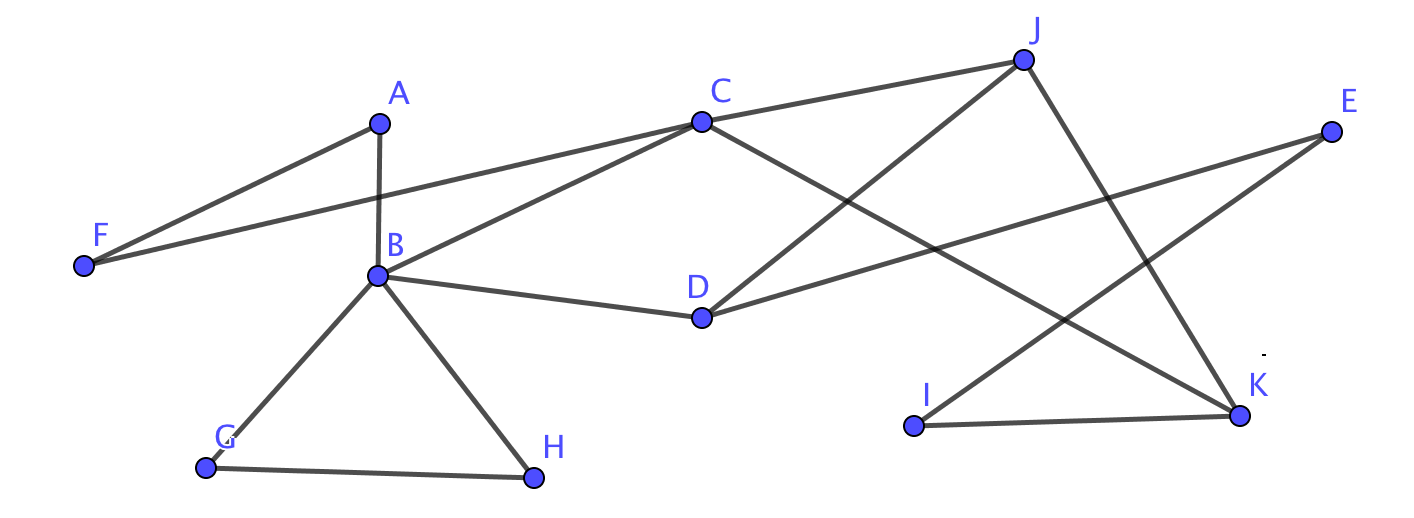
\includegraphics[scale=0.3]{Graph} 

\end{center}
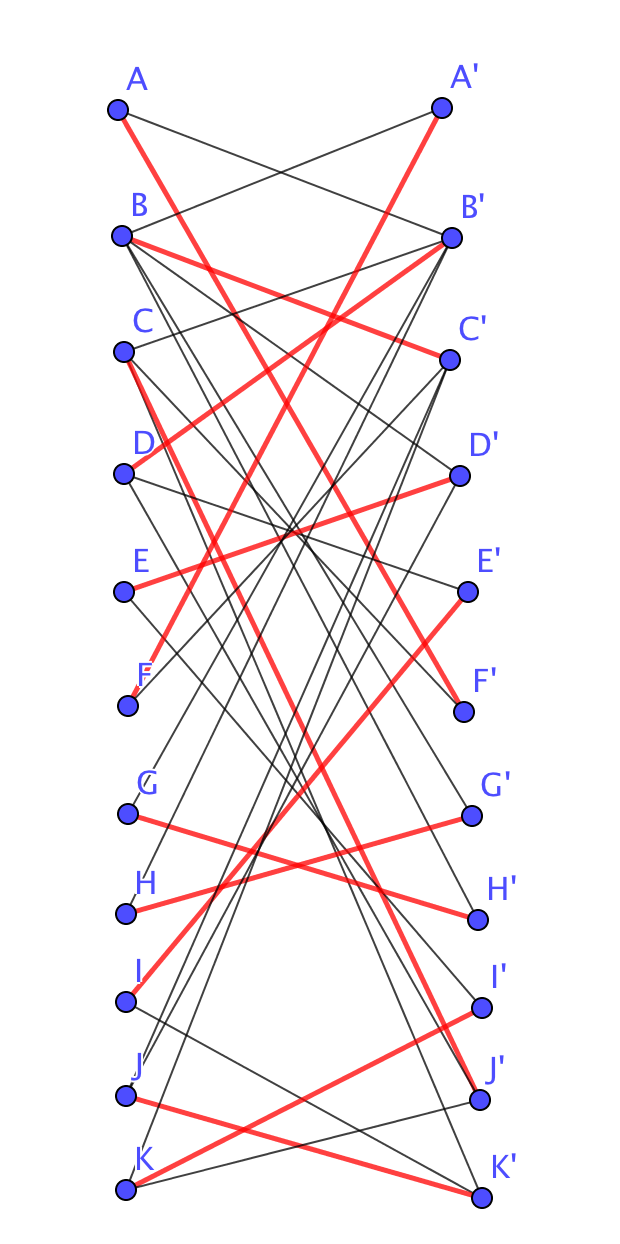
\includegraphics[scale=0.3]{Bipartite} \hfill 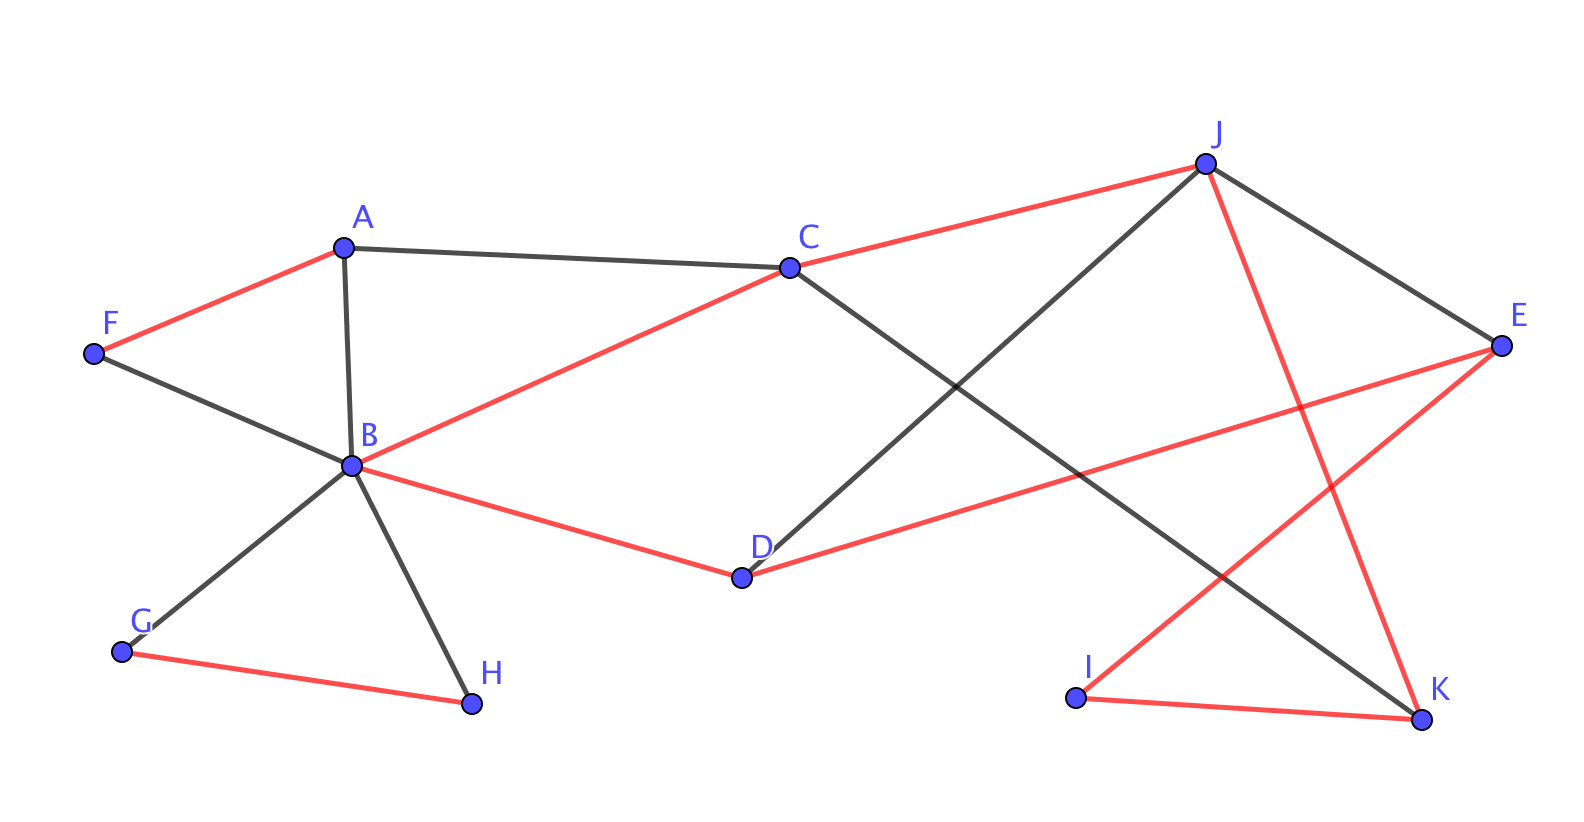
\includegraphics[scale=0.3]{2-matching} 






  \end{document}
